\section{Metodologia}


\begin{frame}{Materiais - Equipamentos e componentes}
\begin{itemize}
\item Microcontrolador de núcleo ARM;
\item Placa de desenvolvimento $Tiva^{TM}$ TM4C123GH6PM (Texas Instruments); 
\item Drive para acionamento do tipo \emph{Pulse Width Modulation} (PWM) com tecnologia CMOS (IRF540);
\item Motor de corrente contínua;
\item Disco compacto (CD);
\item Sensor ótico;
\item Fonte de alimentação chaveada 12V 10W.
\end{itemize}
\end{frame}


%%%%%%%%%%%%%%%%%%%%%%%%%%%%%%%%%%%%%%% Construção do Sistema Físico
\begin{frame}{Construção do Sistema Físico}

\begin{figure}[!htb]
\subfloat[Placa de desenvolvimento]{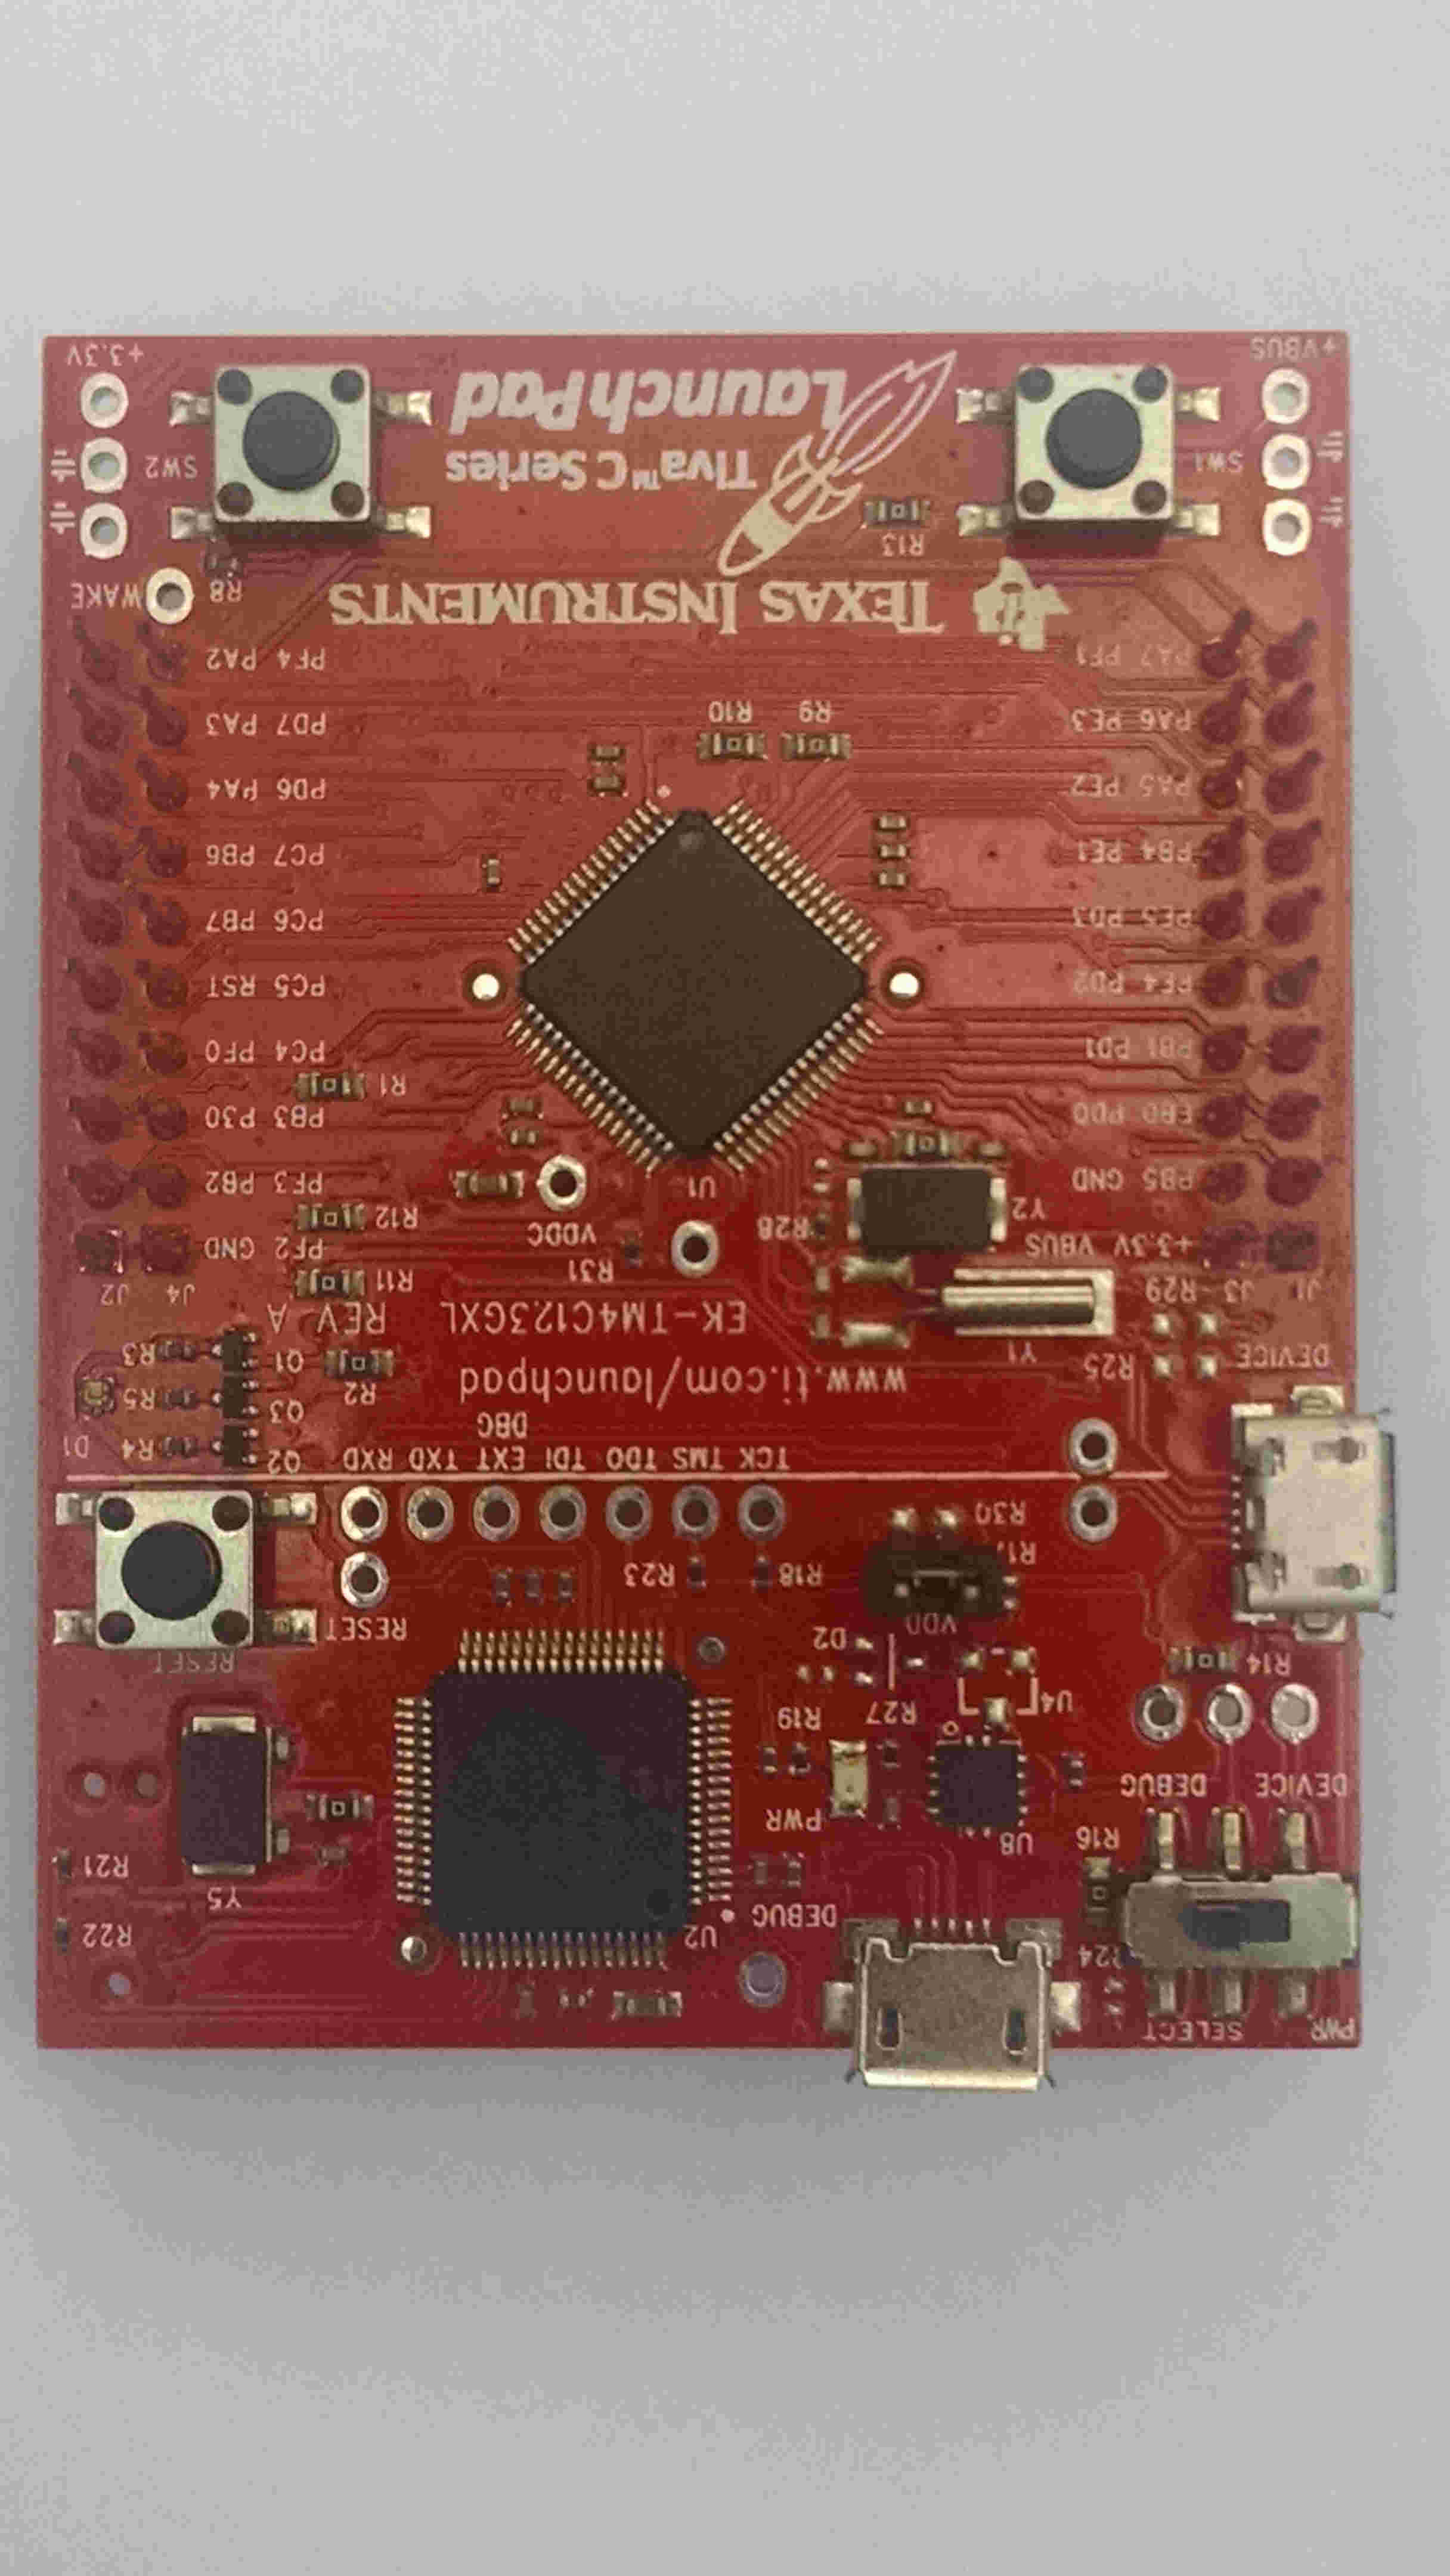
\includegraphics[scale=0.05, angle=180, clip=true, trim=0 750 60 500]{./imagens/uC-ARM.jpg}}
\subfloat[Motor CC]{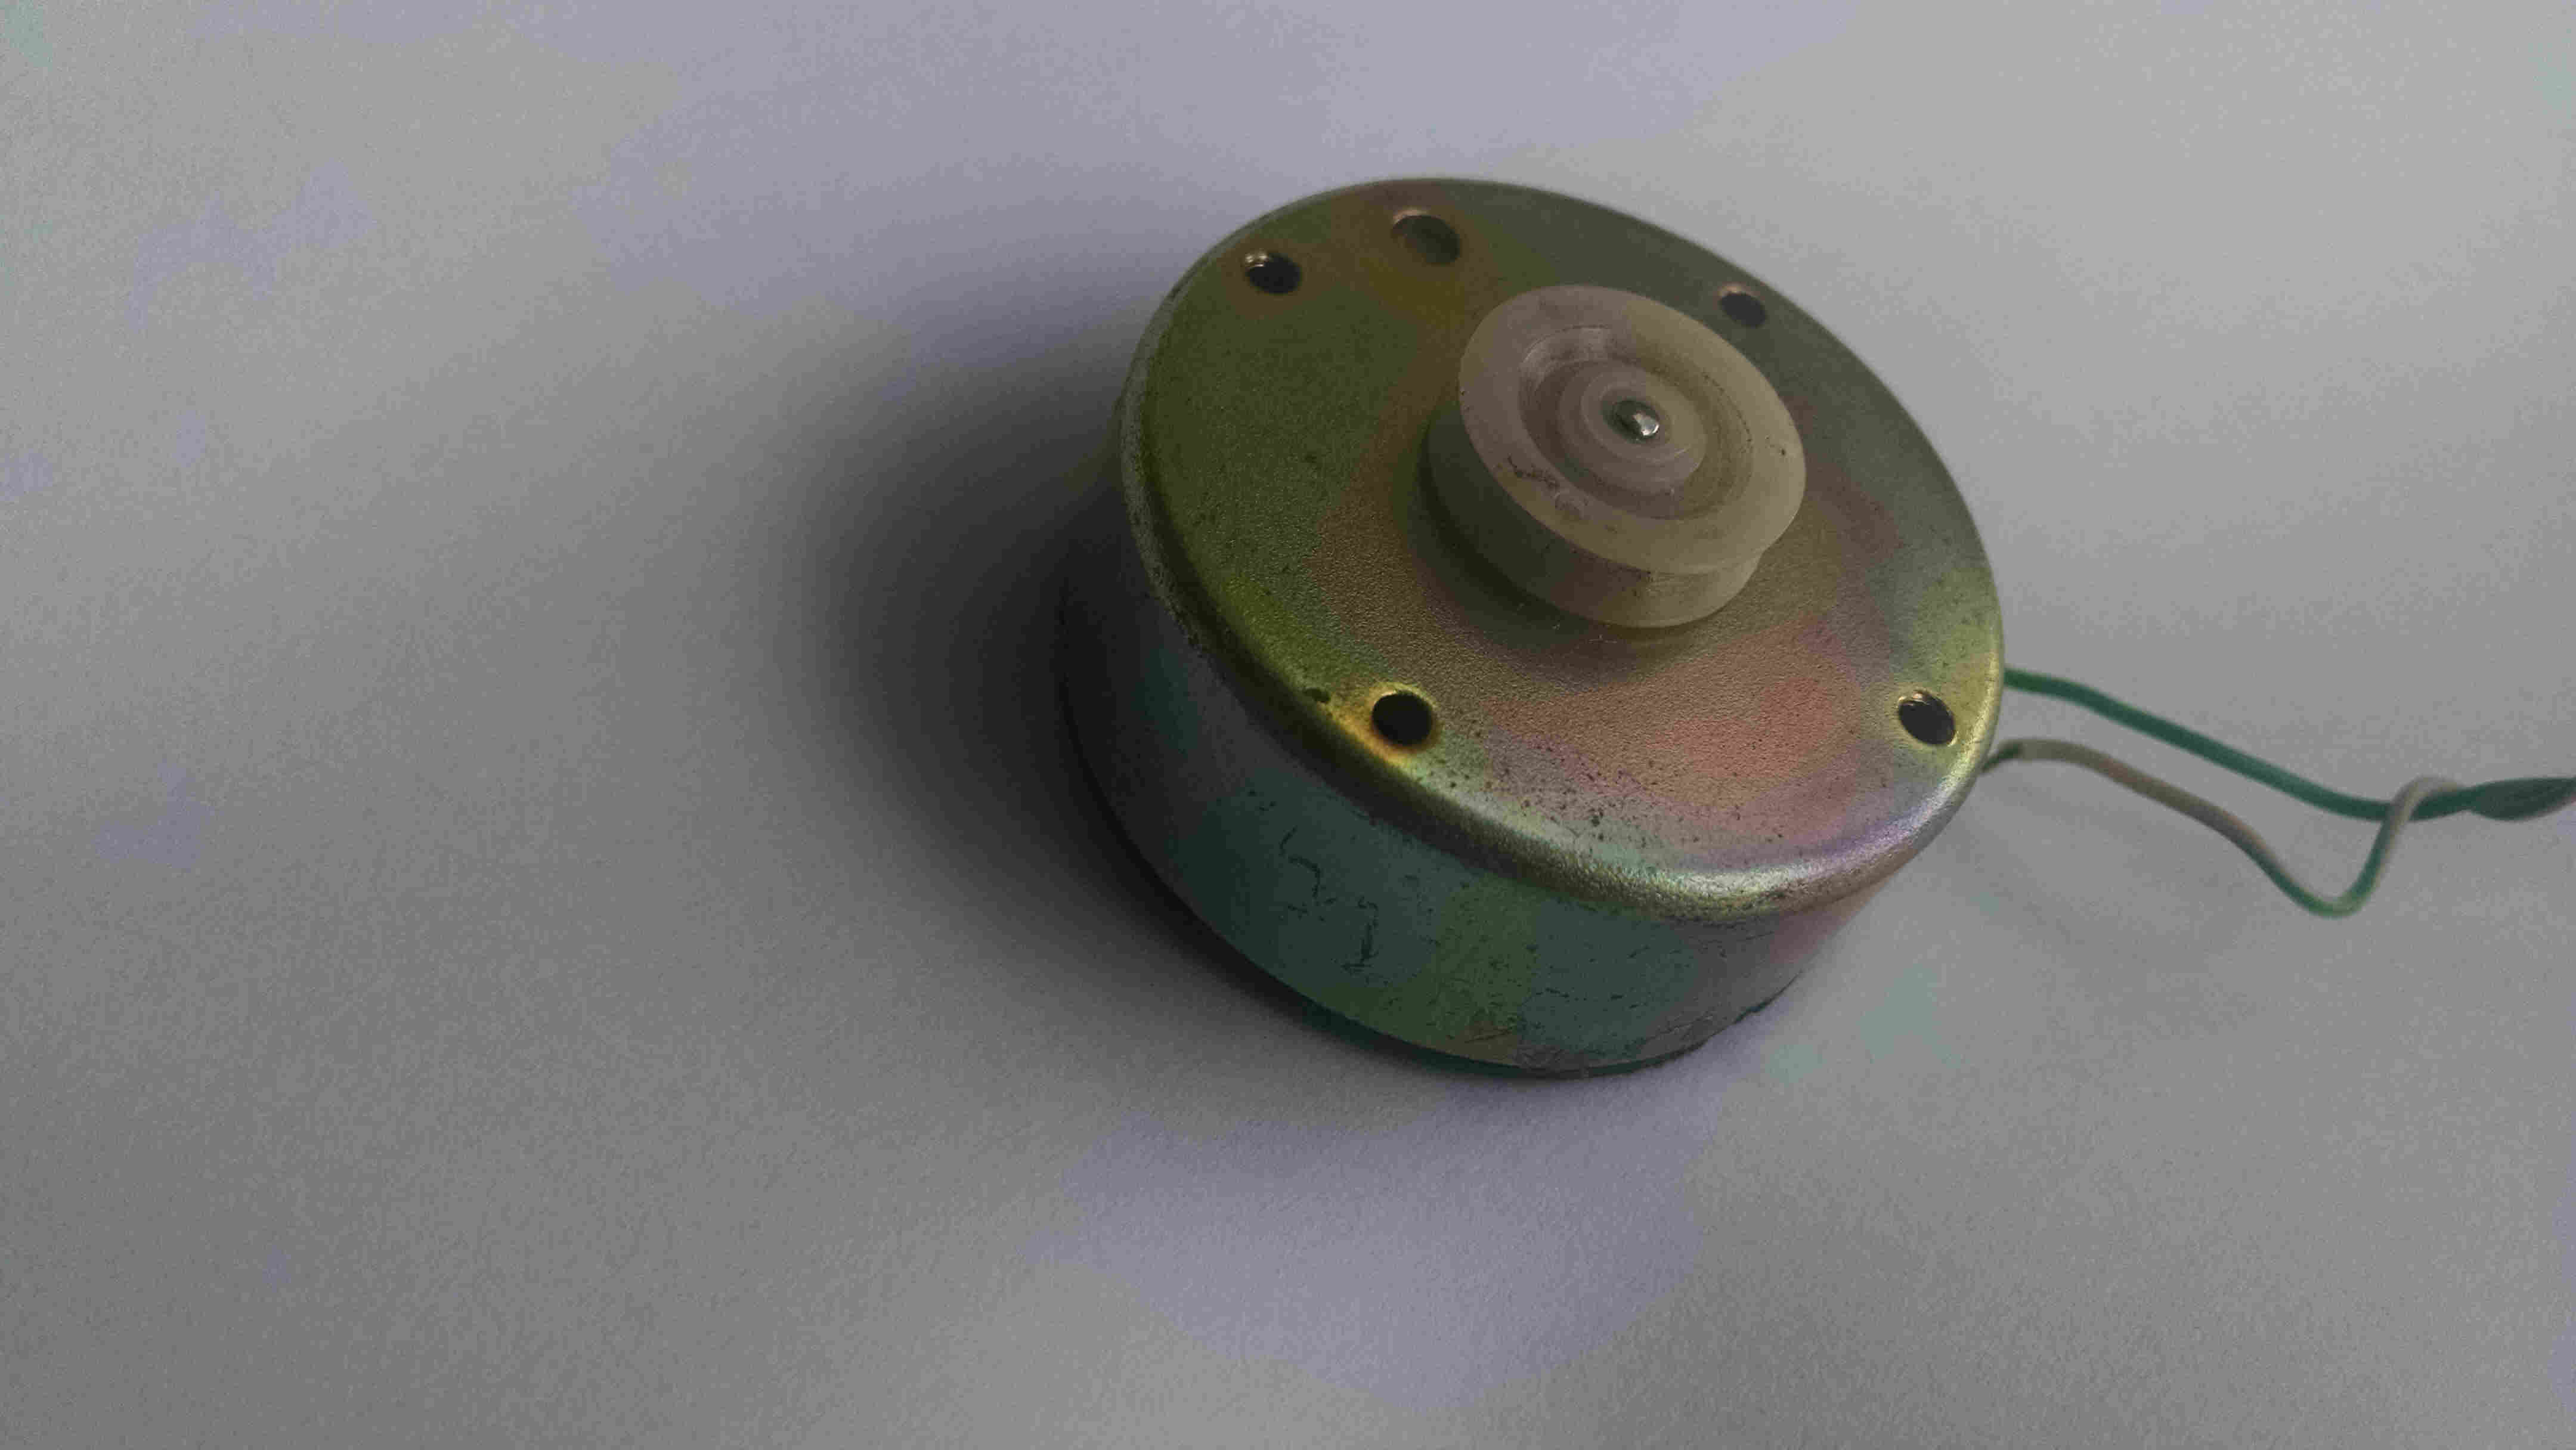
\includegraphics[scale=0.06, angle=180, clip=true, trim=1200 500 600 100]{./imagens/motorDC.jpg}}
\end{figure}

\end{frame}

%%%%%%%%%%%%%%%%%%%%%%%%%%%%%%%%%%%%%%% Sistema construido
\begin{frame}{Sistema construído}

\begin{figure}[!htb]
\subfloat[Sensor de rotação]{ 	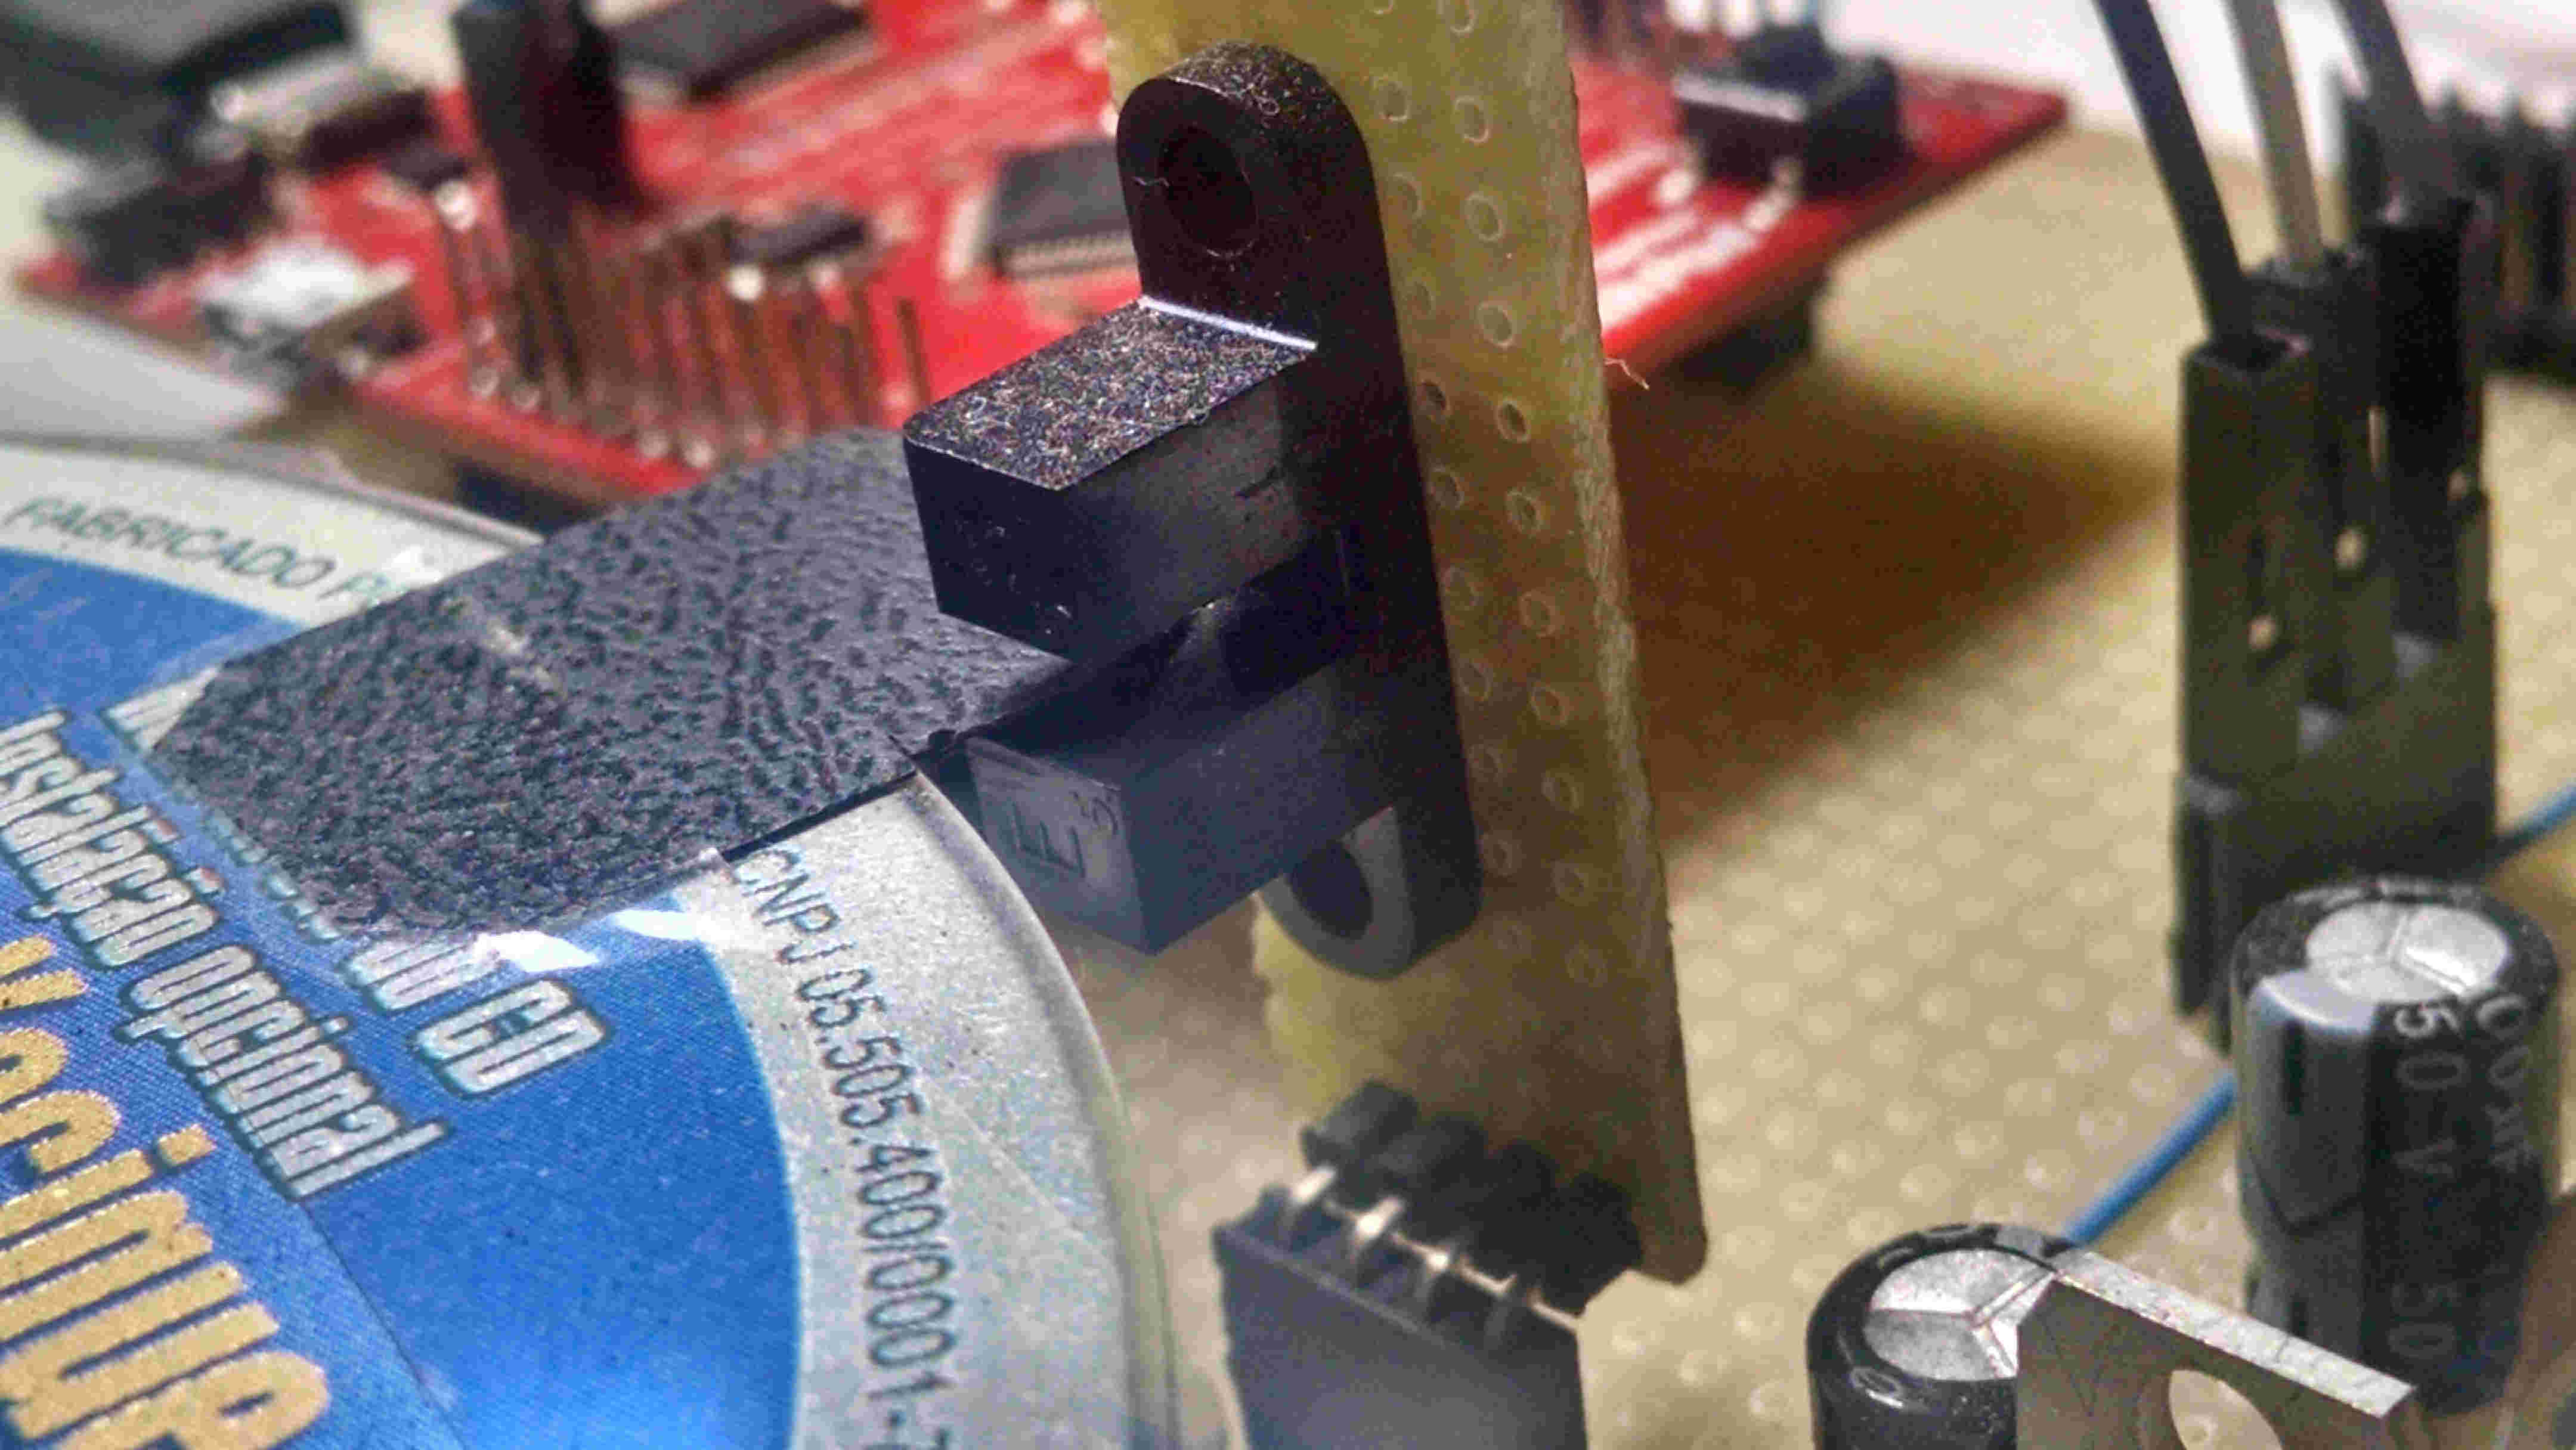
\includegraphics[scale=0.05, angle=0, clip=true, trim=300 200 1200 200]{./imagens/discoSensor.jpg} 	}
\subfloat[Planta de testes]{ 	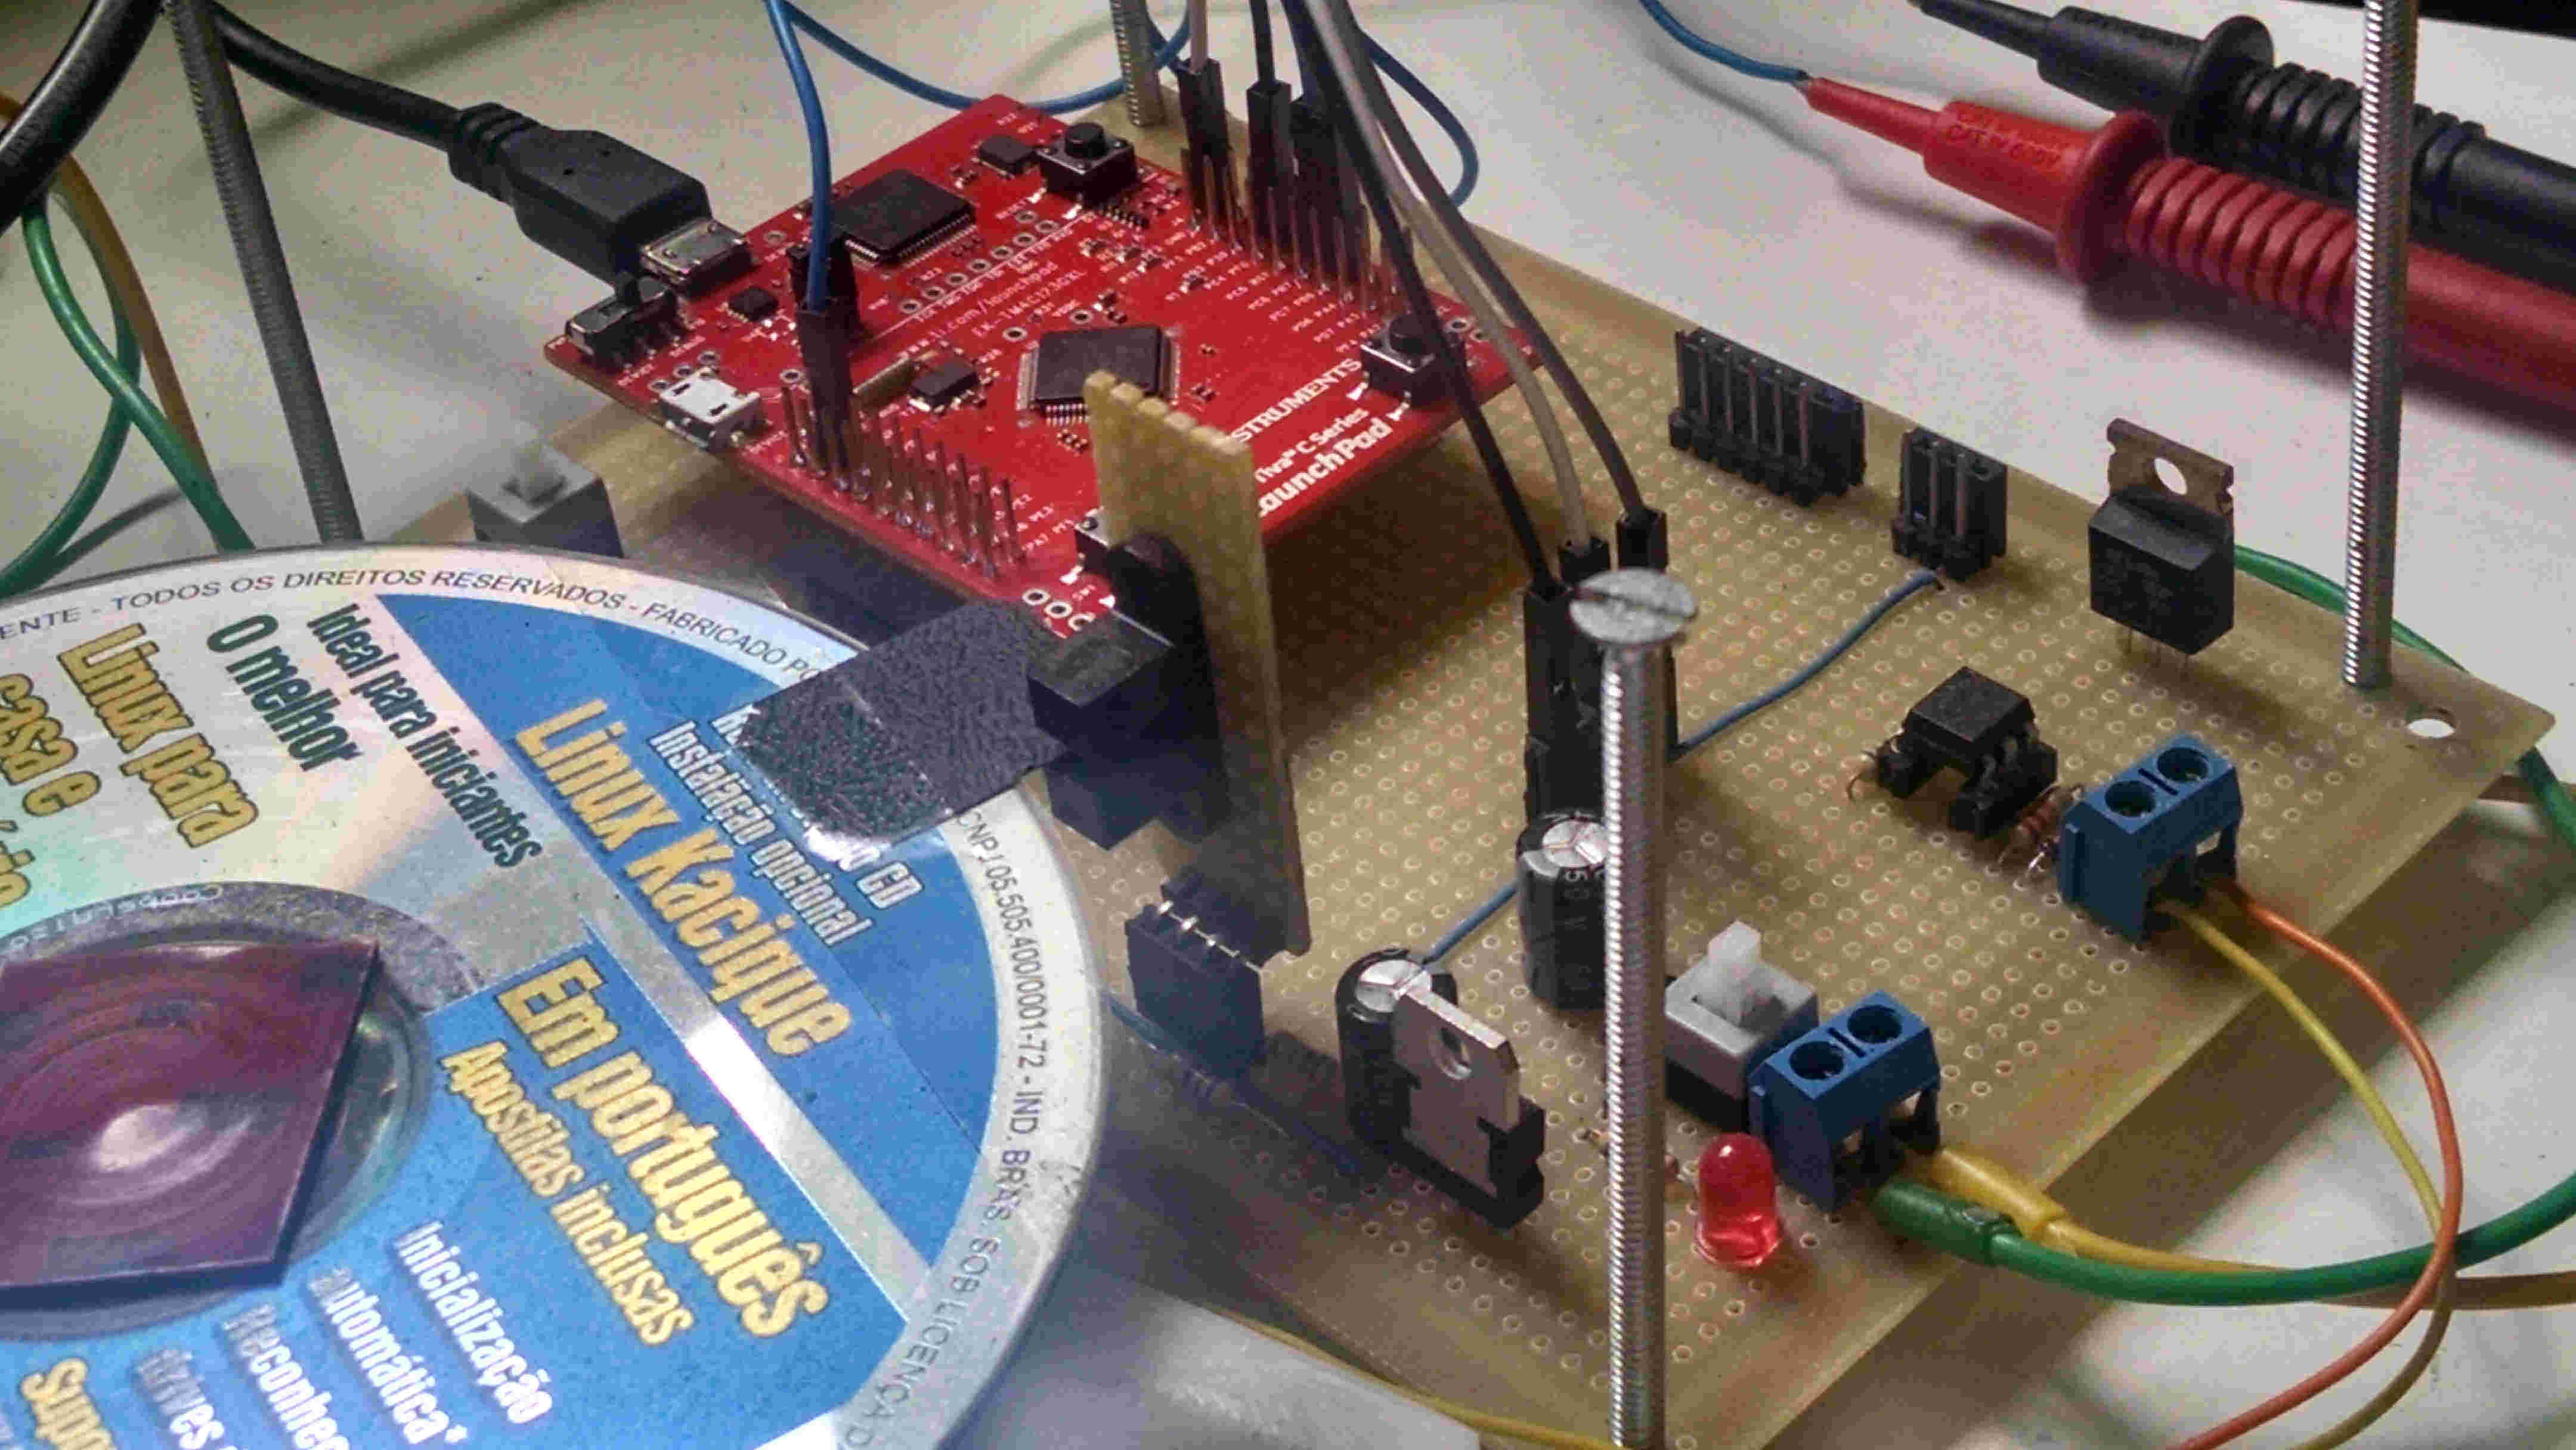
\includegraphics[scale=0.05, angle=0, clip=true, trim=300 200 400 200]{./imagens/discoSensorGeral.jpg} 	}

\end{figure}

\end{frame}


\begin{frame}{Materiais - Ferramentas de software}
\begin{itemize}
\item Sistema Operacional GNU/Linux Debian 8 (Jessie);
\item GNOME Shell;
\item Editores de texto e código fonte: Vim e Emacs;
\item Compilador GCC para ARM (arm-none-eabi-gcc);
\item GNU make;
\item Processador de texto \LaTeX - pdfTEX;
\item Pacotes geradores de figuras TikZ, PGF e GNU pic (Groff);
\item Gerador de gráficos GNUPlot;
\item Terminal de comunicação Minicom;
\item Gravador para microcontrolador ARM LM4Flash.
\end{itemize}
\end{frame}




\begin{frame}{Método}
  \begin{itemize}
    \item Levantamento do modelo matemático do sistema protótipo;
    \item Verificação da qualidade do modelo (erro percentual médio $< 5\%$ );
    \item Definição dos requisitos de desempenho do sistema;
    \item Realizar o controle utilizando um controlador PI;
    \item Realizar o controle utilizando um controlador LPA$E\tau$.
  \end{itemize}
\end{frame}





